\documentclass[11pt]{article}

% basic packages
\usepackage[margin=1in]{geometry}
\usepackage[pdftex]{graphicx}
\usepackage{amsmath,amssymb,amsthm}
\usepackage{custom}

% page formatting
\usepackage{fancyhdr}
\pagestyle{fancy}

\renewcommand{\sectionmark}[1]{\markright{\textsf{\arabic{section}. #1}}}
\renewcommand{\subsectionmark}[1]{}
\lhead{\textbf{\thepage} \ \ \nouppercase{\rightmark}}
\chead{}
\rhead{}
\lfoot{}
\cfoot{}
\rfoot{}
\setlength{\headheight}{14pt}

\linespread{1.03} % give a little extra room
\setlength{\parindent}{0.2in} % reduce paragraph indent a bit
\setcounter{secnumdepth}{2} % no numbered subsubsections
\setcounter{tocdepth}{2} % no subsubsections in ToC

\begin{document}

% make title page
\thispagestyle{empty}
\bigskip \
\vspace{0.1cm}

\begin{center}
{\fontsize{36}{36} \selectfont \bf \sffamily Housing Notes}
\vskip 24pt
{\fontsize{18}{18} \selectfont \rmfamily Conor Redington} 
\vskip 24pt
\end{center}

{\parindent0pt \baselineskip=15.5pt \lipsum[1-4]}

% make table of contents
\newpage
\microtoc
\newpage

% main content
\hypertarget{housing}{%
\section{Housing}\label{housing}}

@economics @housing @ireland

\emph{The goal here is to constantly update this document by making
claims and doing reading to edit those claims}

\hypertarget{why-housing-in-ireland-is-so-expensive}{%
\section{Why Housing in Ireland is so
expensive}\label{why-housing-in-ireland-is-so-expensive}}

\begin{itemize}
\tightlist
\item
  The government are lobbied by institutional investment firms so they
  can buy up all the houses and hold them increasing their price
  artificially.
\end{itemize}

What does it take for this to be true.

\begin{itemize}
\tightlist
\item
  Evidence of government interest in institutional investment in housing
  and/or general interest in rising house prices.
\item
  Evidence of constraining supply artificially to increase a firms
  profits.
\end{itemize}

\hypertarget{section}{%
\section{08/04/23 14:05:49}\label{section}}

\emph{Following Karnofsky method}

Step 1: pick a topic. First, I decide what I want to form an opinion
about. My basic approach here is: ``Find claims that are important if
true, and might be true.''

Step 2: read and/or discuss (a bit). I usually start by trying to read
the most prominent 1-3 pieces that (a) defend the claim or (b) attack
the claim or (c) set out to comprehensively review the evidence on both
sides

Step 3: explain and defend my current, incredibly premature hypothesis,
in writing (or conversation).

Step 4: find and list weaknesses in case.

I think what might be useful is to construct some `stakeholder'
profiles/takes on the current situation that I think are out there. Then
try and get evidence to back each one.

\emph{Try and focus on statements that have an effect on outcome}

\hypertarget{step-1-current-viewclaims}{%
\subsection{Step 1 Current
view/claims}\label{step-1-current-viewclaims}}

\begin{itemize}
\tightlist
\item
  Housing supply in Ireland is low due to construction costs and land
  regulation. Land tax should be instituted along with more data on
  construction value chain to reduce its costs.
\item
  Institutional investors are a small portion of the housing market
  (buying and selling of housing) and of the rental market (letting).
\item
  The way out is to incentivise more private funding to meet demand in
  all it's diversity. That is, the government would be too slow an
  organization to meet the changing demand and would make things worse.
\item
  The government can not afford to meet housing need. Supply is
  currently way below demand.
\end{itemize}

\hypertarget{step-2-readdiscuss-major-pieces}{%
\subsection{Step 2 read/discuss major
pieces}\label{step-2-readdiscuss-major-pieces}}

\begin{itemize}
\tightlist
\item
  `Housing for All' is the government's housing plan to 2030.

  \begin{itemize}
  \tightlist
  \item
    Jesus, literally all my claims are on p.16. Did I nail it?
  \item
    ``Ireland needs on average 30,000 new homes per annum to meet
    targets set out for additional households as outlined in the
    National Planning Framework''.
  \item
    Four pathways for overarching objectives with 20bn for them all over
    5 years.

    \begin{itemize}
    \item
      \begin{enumerate}
      \def\labelenumi{\arabic{enumi})}
      \tightlist
      \item
        Supporting Home Ownership and Increasing Affordability
      \end{enumerate}

      \begin{itemize}
      \tightlist
      \item
        Increase new housing supply to 33,000 per year up to 2030.
      \item
        6,000 affordable homes to be made available to rent or buy per
        year from AHB's, Local Authorities or LDA.
      \item
        Introduction of cost rental homes and indefinite leases.
      \item
        LDA will start building more on state land and will advance
        Project Tosaigh.
      \end{itemize}
    \item
      \begin{enumerate}
      \def\labelenumi{\arabic{enumi})}
      \setcounter{enumi}{2}
      \tightlist
      \item
        Increasing Housing Supply
      \end{enumerate}

      \begin{itemize}
      \tightlist
      \item
        ``To build housing, we need land. This land needs to be serviced
        with transport, utilities and other infrastructure''
      \item
        ``The overall investment required to build an average of 33,000
        homes per year is estimated at €12bn.''
      \end{itemize}
    \end{itemize}
  \item
    In terms of modelling, the Scottish housing need model is the
    leader.
  \item
    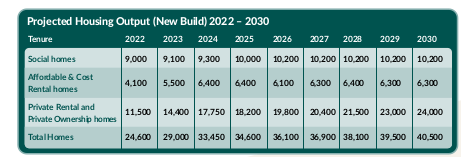
\includegraphics{img/housingdemandhndamodel.png}
  \end{itemize}
\end{itemize}

If we just focus on the housing supply claim for now. Pathways 1 and 3
are directly related to that.

\hypertarget{profiles}{%
\subsection{Profiles}\label{profiles}}

\begin{itemize}
\tightlist
\item
  ``Housing is being `held back' to increase it's price''
\item
  ``Institutional invested buy up all the housing stock and do the
  above''
\item
  ``There is not enough affordable housing''
\item
  ``The government could just build all the houses we need.''
\item
  ``The government do not care, nothing is being done''
\end{itemize}

What am I really arguing over here? What are the claims. It seems my
goal is to have a full picture of the nuance involved but I'd also like
to be able to assign some blame, I suppose, as to why were in this
situation in the first place.

\hypertarget{gather-all-notes}{%
\section{Gather all notes}\label{gather-all-notes}}

\hypertarget{affordable-housing}{%
\subsection{Affordable housing}\label{affordable-housing}}

\begin{itemize}
\tightlist
\item
  The guiding principle in affordable housing finance is that public and
  private financing sources must equal uses or the total cost of
  building the building, also know as development cost
\item
  In Ireland approved housing bodies seem to be supported by Housing
  Finance Agency. The question then becomes how much supply can these
  not for profits really provide.
\end{itemize}

\hypertarget{why-cant-we-just-mandate-non-profit-developers}{%
\subsection{Why can't we just mandate non profit
developers}\label{why-cant-we-just-mandate-non-profit-developers}}

\begin{itemize}
\tightlist
\item
  for profit is fundamental to capitalism. Debating for profit debates
  the incentives of capitalist economy.
\item
  Socialist housing may not agree with the general populace (high
  taxes), also, it may not be efficient (in terms of the types of
  housing provided)
\end{itemize}

\hypertarget{demand-demographics}{%
\section{Demand Demographics}\label{demand-demographics}}

What kind of housing are people asking for?

\begin{itemize}
\item
  \begin{quote}
  Figures from the most recent Census, undertaken in 2016, show that
  18\% of households rent their home from a private landlord, while a
  further 8\% rent from a Local Authority or an Approved Housing Body
  \end{quote}
\item
  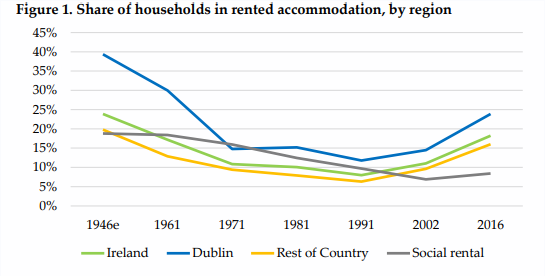
\includegraphics{img/shareofhouseholdsinrental.png}
\item
  In a generation the share in rental accomadation has almost doubled.
\end{itemize}

\hypertarget{first-principles}{%
\section{First principles}\label{first-principles}}

\begin{itemize}
\tightlist
\item
  How much does a typical house cost?

  \begin{itemize}
  \tightlist
  \item
    Types of houses
  \item
    Cost (average or breakeven) of each type of house, in Dublin and the
    rest of Ireland
  \end{itemize}
\item
  Social housing
\item
  Why can't the government fund the whole thing?

  \begin{itemize}
  \tightlist
  \item
    How much money does the government have?
  \item
    How long does it take to build a house through public means?
  \end{itemize}
\end{itemize}

\hypertarget{reading}{%
\subsection{Reading}\label{reading}}

\begin{itemize}
\tightlist
\item
  https://www.ucd.ie/geary/static/publications/workingpapers/gearywp201901.pdf
\item
  https://www.irishtimes.com/news/social-affairs/a-century-of-housing-how-the-state-built-ireland-s-homes-1.3785939
\item
  https://catuireland.org/i-like-public-housing-and-so-should-you/
\item
  \href{https://mises.org/wire/why-we-need-landlords}{argument for the
  existence of landlords}
\item
  \href{https://www.urban.org/urban-wire/how-affordable-housing-gets-built}{How
  affordable housing gets built}

  \begin{itemize}
  \tightlist
  \item
    https://apps.urban.org/features/cost-of-affordable-housing/
  \end{itemize}
\item
  https://www.oecd.org/housing/topics/affordable-housing/
\item
  \href{./../../vimwiki/Housing\%20Market\%20Course.md}{housing course}
\item
  \href{https://irp.cdn-website.com/4065c16c/files/uploaded/Identify\%20Consulting\%20June\%202021\%20PRS\%20Report\%20for\%20IIP\%20-\%20final.pdf}{Lyons
  2021}
\item
  \href{https://publicpolicy.ie/perspectives/understanding-irelands-housing-challenge-in-the-light-of-housing-for-all/}{Understanding
  Irelands Housing challenge}

  \begin{itemize}
  \tightlist
  \item
    Interesting to note how Irelands policy just flipped to home
    ownership as the goal from the rental sector in the previous major
    policy
  \item
    The large amount of institutional investment in irelands residential
    investment goes into build to rent. We seem to need more investment
    from abroad as we can not fund it ourselves but this brings with it
    this supply of btr.
  \item
    There's also a supply deficit. It seems that around 50,000 dwellings
    should be built a year for projected Irish population growth. The
    target for Housing for All is 30,000.
  \item
    It is not clear if the decline in home ownership is due to supply
    shortage. Credit conditions could also play a role
  \end{itemize}
\item
  \href{https://www.cluid.ie/wp-content/uploads/2021/04/WEB-Cluid-Housing-Towards-a-Sustainable-Rental-Sector-in-Ireland-Understanding-the-Key-Challenges-and-Opportunities.pdf}{KPMG
  report}

  \begin{itemize}
  \tightlist
  \item
    To cope with a rise in demand for housing from economic growth in
    the early 90's the Urban renewal act allowed landlords to write off
    100\% of costs on their income tax, this was only 50\% in the case
    of owner occupied landlords. This lead to 60\% of subsidies units
    being owned by private landlords.
  \item
    Despite these incentives ending in the mid 2000's cheap credit
    propped the development market up.
  \item
    Home ownership for 25-34 year olds has declined from 68\% in 1991 to
    30\% in 2016
  \item
    There this changing landscape for demand, is policy then playing
    catch up?
  \end{itemize}
\item
  \href{https://www.ucd.ie/geary/static/publications/workingpapers/gearywp201901.pdf}{Golden
  age of Irish social housing}

  \begin{itemize}
  \item
    \begin{quote}
    Until recently almost all social housing in Ireland was delivered,
    owned and managed by local government, but apart from the United
    Kingdom, this model was rarely used elsewhere. In the rest of
    Western Europe social housing was provided by the independent,
    non-profit sector organisations (eg. cooperatives in Denmark,
    housing associations in the Netherlands and Austria),
    quasigovernmental municipal housing companies (in France and Sweden)
    or less commonly the private sector (Germany)
    \end{quote}
  \item
    Coincided with the expansion of the welfare state
  \item
    Services of housing loans became an issue
  \item
    Funding of debt through rents.
  \item
    Debt held by non profit agencies in other Western countries
  \item
    Ireland financing was destabilised by politics
  \end{itemize}
\item
  https://www.irishtimes.com/news/social-affairs/a-century-of-housing-how-the-state-built-ireland-s-homes-1.3785939
\end{itemize}

\hypertarget{notes}{%
\section{Notes}\label{notes}}

\begin{itemize}
\tightlist
\item
  \href{https://irp.cdn-website.com/4065c16c/files/uploaded/Identify\%20Consulting\%20June\%202021\%20PRS\%20Report\%20for\%20IIP\%20-\%20final.pdf}{Lyons
  2021}

  \begin{itemize}
  \item
    At the end of 2.1 there is a discussion of the `path dependence' of
    irish housing based on financing model. Analyses in Blackwell and
    Kohl (2008)
  \item
    Ireland is converging demographically to the EU average in terms of
    population growth and the no. of apartments
  \item
    Two thirds of landlords in a survey commissioned by the RTB own just
    one property.
  \item
    \begin{quote}
    For almost all of the 19th century, there were no purpose-built
    apartments constructed in Ireland. This and the later absence of
    apartment construction reflects a unique element of Ireland's
    demographic development: unlike all our European peers, Ireland's
    population fell, rather than increased rapidly, between the mid-19th
    and mid20th century. This meant there was, effectively, no pressure
    on either the policy or finance systems to plan how to accommodate
    density: instead, sparser and more sprawled greenfield development
    was sufficient
    \end{quote}
  \item
    There was virtually no private rental accomadation built at the
    start of the 20th century in Ireland due to viability (which I think
    means that the market price wasn't even enough to cover costs). Most
    building was subsidised and suburban due to transport infrastruce
    slowly being set up.
  \item
    An example is given of the disparity between the market price and
    costs of development even in the 60's. It is similar to today, where
    incomes just can't match the break even price.
  \item
    Ireland followed the European trend post war to build pre caste
    large scale developments (liek Ballymun) later following what other
    countries do mixing tenures (in terms of market renters and social
    renters together)
  \item
    In the 80's the government tried to deal with the lack of viability
    for capital with a 40\% subsidy for cost of developments
  \item
    Under section 23 you could get the cost of building minus the site
    cost off the income you made from rent. So anything you built would
    contribute towards you not having to pay tax on the rent you earned
    from it. This was also aggregate rental income. You could be
    building houses that there were no demand for but getting a huge tax
    break on the income you were making from somewhere else.
  \item
    This seems to have worked as rents decreased after it's
    implementation
  \item
    This tax break only applied to private taxpayers which meant that
    institutional investors were essentially priced out?
  \item
    2.3
  \item
    2.4

    \begin{itemize}
    \tightlist
    \item
      Institutional investors play an important role in build to rent
      projects as they have access to longer term capital from European
      markets. Like pension funds. This means they can spread the costs
      of construction over a longer period of time.
    \item
      This is frowned upon in Ireland as it's seen as `squeezing out'
      the regular developer(?). How else would this accomadation be
      built?
    \end{itemize}
  \end{itemize}
\item
  Lyons 2021 continued

  \begin{itemize}
  \tightlist
  \item
    Sales prices of housing are about 40\% below 2007 peak. Being around
    20\% below in Dublin
  \item
    Rental prices are 40\% above their peak though
  \item
    Show's scatterplots that link increases in supply with reduction in
    rent and vice versa. The equilibrium seems to be above 4,000 units
    available
  \item
    Interesting how this is the largest rental boom in modern history,
    I'm not too sure what the cause of the others were.
  \item
    I skipped 3.1, assumptions for growth and expected housing need.
  \item
    3.2

    \begin{itemize}
    \tightlist
    \item
      Almost 80\% of developments use foreign captial. Either in equity
      or debt form.
    \item
      My mental model here for equity is some firm that is `investing'
      in a development rather than just expecting their money back.
    \item
      Interesting that during the tiger the `pillar banks' played a
      large role in capital circulation. That now they are more
      restrained so it was inevitable that some other form of capital
      must come in. Also, they were intermdeiaries for foreign capital.
      So the money you were getting from the bank was just coming from
      overseas anyways 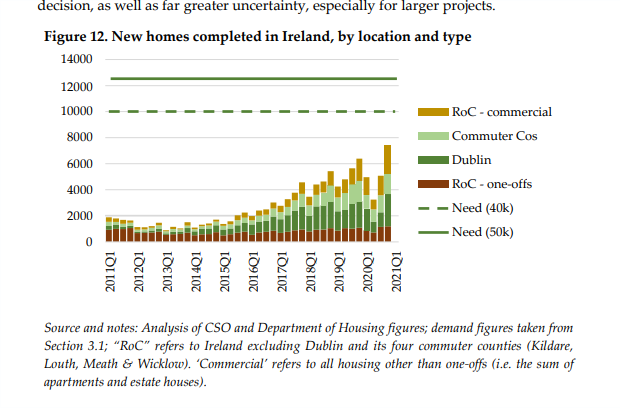
\includegraphics{img/chart.png}
    \item
      It's made how short need we are
    \end{itemize}
  \item
    What is the government expenditure profile like in the past few
    years. Why do we need international capital
  \end{itemize}
\item
  \href{file:///home/conor/Downloads/205477_d744837d-8f03-4ff0-82dd-4763df823c95.pdf}{local
  file}

  \begin{itemize}
  \item
    This report seems to talk more about economic cylces and how they
    affect social housing, which I think is an interesting point.
  \item
    \begin{quote}
    Rising rents can also increase the cost faced by the exchequer in
    providing housing. With regard to housing measures funded through
    current expenditure, a large share of the rental sector in Ireland
    is in receipt of some form of support. Data from the 2016 census
    indicates that 326,8324 households rent from a landlord (including
    voluntary and co-operative bodies). As of 2021Q2, there were
    approximately 62,000 active HAP tenancies, 17,500 RAS tenancies, and
    5,000 privately leased SHCEP operational units (DHLGH). This
    indicates that approximately 26\% of households residing in the
    rental sector are in receipt of some form of housing support that is
    funded through current expenditure.
    \end{quote}
  \item
    Be interesting to check this for the most recent census.
  \item
    Interesting point on how more strict mortgage lending rules affect
    price signals and push people to the rental sector, so rent increase
    more than avg. house prices.
  \item
    \begin{quote}
    Census data indicates that the age at which home ownership became
    the majority tenure category was 35 years in
    \end{quote}

    \begin{enumerate}
    \def\labelenumi{\arabic{enumi}.}
    \setcounter{enumi}{2015}
    \tightlist
    \item
      Below the age of 35, the number of households renting exceeded
      those owning a home. Previous censuses indicate the ages which
      have marked the changeover between renting and homeownership; 32
      (2011), 28 (2006), 27 (2002), 26 (1991)
    \end{enumerate}
  \end{itemize}
\end{itemize}

\end{document}
